%% Revisado por Gabriel Saraiva
%% Revisado por Renata

\chapter{Revisão Bibliográfica}
\label{cap2}


Neste capítulo são apresentados os conceitos sobre Sistemas de Arquivos Distribuídos (com foco na comunicação entre cliente e servidor), e principalmente dispositivos móveis, apresentando suas restrições.


\section{Sistemas Distribuídos}

    Segundo ~\cite{tanenbaum}, um Sistema Distribuído (SD) é um conjunto de computadores independentes que se apresenta aos usuários como um sistema único e coerente, ocultado detalhes da implementação que não são úteis aos usuários. Ainda sim um sistema distribuído pode ser definido de acordo com ~\cite{coulouris} como um sistema onde os componentes computacionais, tanto os de \textit{hardware} como os de \textit{software}, se comunicam e coordenam suas ações através de mensagens transmitidas por uma ou mais redes de computadores, independente da distância entre seus componentes. Essas características, agregam diversos desafios na implementação de sistemas distribuídos. De acordo com ~\cite{coulouris} esses desafios são:
    
    \subsection{Heterogeneidade}
        Como esses sistemas muitas vezes são compostos por \textit{hardwares} e arquiteturas diferentes, diversos sistemas operacionais e \textit{softwares} desenvolvido por diferentes equipes e muitas vezes com configurações distintas entre outros fatores. Dessa forma é de grande importância que todo o sistema seja baseado em protocolos compatíveis que possam gerenciar essas diferenças e fornecer ao usuário um ambiente único e coeso.
    
    \subsection{Abertura}
        Um sistema é dito aberto quando suas interfaces de comunicação ou de desenvolvimento são acessíveis e programas podem ser feitos ou alterados por terceiros para que sejam compatíveis com esse sistema. Os grandes desafios para criar sistemas abertos são: fornecer principais interfaces publicamente, mecanismos de comunicação uniforme para acesso a recursos compartilhados e por fim, realizar os testes necessários para que esse sistema se comporte como esperado e seja compatível com o padrão publicado.
    
    \subsection{Segurança}
Um dos grandes desafios de sistemas distribuídos é manter a segurança do próprio sistema de modo a manter a disponibilidade do serviço a seus clientes, confidencialidade dos dados que ele armazena ou processa e não menos importante a integridade do sistema e dos dados que estão no SD. Esse tópico é de grande importância na maioria dos SD disponíveis pois afeta principalmente a disponibilidade do serviço aos usuários e a confiança que o usuário tem sobre o serviço ~\cite{coulouris}.
    
    \subsection{Escalabilidade}
        Um sistema é dito escalável se seu desempenho cresce proporcionalmente aos recursos que são inserido no SD, sem perda de qualidade ou desempenho do serviço. Essa característica é muito importante para que o sistema continue operando em cenários que exijam mais recursos do que o cenário inicial para o qual o sistema implantado. Embora pareça um desafio fácil de solucionar, como mostrado em ~\cite{coulouris}, as soluções desses desafios não são sempre triviais, como por exemplo gerenciar a perda de desempenho do sistema ao aumentar o número de servidores e clientes em uma rede, ou manter a latência dentro de um patamar aceitável com o crescimento do número de servidores e a distância entre eles.
    
    \subsection{Tratamento de falhas}

        Como o sistema é distribuído, falhas tendem a não comprometer a totalidade do sistema, afetando apenas alguns pontos  por vez enquanto outros continuam operando. Mas isso torna essas falhas complexas de serem tratadas, para que o sistema volte a operar como esperado ~\cite{coulouris}. Para tratar essas falhas são utilizadas as seguintes técnicas:
        \begin{enumerate}
    
            \item Detecção de falha: Erros de transmissão por exemplo podem ser detectados e facilmente corrigidos através de mecanismos próprios e algoritmos bem conhecidos como por exemplo o os algoritmos de \textit{hash} \textit{Message-Digest algorithm 5} (MD5) e o \textit{Secure Hash Algorithm} (SHA);
            
            \item Mascaramento de falha: Essa técnica consiste não em solucionar o problema mas aumentar a resistência do sistema as falhas, como por exemplo replicar informações servidores e retransmitir mensagens danificadas;
            
            \item Tolerância a falhas: Nem sempre é possível construir sistemas a prova de falhas, sendo muito mais simples e barato projetá-los para tolerar algumas falhas até certo ponto e depois disso informar o usuário sobre a falha ocorrida. Um exemplo clássico citado em ~\cite{coulouris} é o do navegador \textit{web} que, após um certo número de tentativas sem sucesso de carregar uma página \textit{web}, desiste de tentar carregar a página e informa o erro ao usuário;
            
            \item Redundância: Outra forma de tornar o sistema mais tolerante a falhas é acrescentar redundância ao sistema, para que caso uma parte falhe, outras partes detectem essa falha e assumam as tarefas do módulo que falhou sem prejudicar o funcionamento do sistema como um todo. Exemplos são servidores replicados e múltiplas rotas para um destino ~\cite{coulouris};
            
            \item Recuperação de falhas: Mesmo que não seja possível evitar falhas, é importante que o sistema seja capaz de se recuperar delas. Um exemplo disso é o uso de \textit{logs} nos sistemas de arquivos locais e de servidores que fazem sincronismo com seus pares após alguma falha que cause a falta de sincronismo do sistema ~\cite{coulouris};
            
        \end{enumerate}
    
    
    \subsection{Transparência}
    
        Dentre diversos recursos para fornecer um sistema coerente ao usuário e esconder dele a complexidade do sistema, estão os conceitos de transparência. Como apresentado em ~\cite{tanenbaum}, é possível listar os conceitos de transparência que o projeto atual utiliza de forma mais intensiva, como por exemplo:
    
        \begin{itemize}
            \item Transparência de acesso: toda a complexidade no acesso dos dados é escondida do usuário;
            
            \item Transparência de localização: oculta do usuário a localização dos recursos distribuídos;
            
            \item Transparência de migração: é responsável por omitir do usuário detalhes referente a migração dos dados para outras localidades físicas e lógicas;
            
            \item Transparência de replicação: ocultam do usuário os mecanismos de replicação dos dados;
            
            \item Transparência de falhas: esconde do usuário e tenta solucionar os problemas referentes as falhas que ocorrem no sistema, de modo a evitar com que o usuário seja prejudicado quando uma falha acontece no sistema, como visto anteriormente, detectando, mascarando, tolerando, usando módulos redundantes ou até mesmo recuperando o sistema quando possível.
        \end{itemize}
    
        Embora todas essas camadas de transparência sejam desejadas nem sempre é possível fornecer transparência total ao usuário por questões práticas, como usabilidade, complexidade na implementação e a degradação do desempenho que elas geram.

\section {Sistema de Arquivos}
    Sistemas de arquivos (SA) foram criados para oferecer ao programador uma interface padronizada de acesso aos arquivos, independente de como e onde estão armazenados ~\cite{coulouris} dentro dos dispositivos locais. 
    Além dos dados (arquivos propriamente ditos), sistemas de arquivos devem armazenar também os metadados, que são informações sobre os dados (arquivos). Esses metadados comumente são os seguintes ~\cite{coulouris} (adaptado):
    
    \begin{itemize}
        \item Nome do arquivo;
        \item Dono do arquivo;
        \item Grupo do arquivo;
        \item Horário de criação;
        \item Horário de acesso;
        \item Horário de modificação;
        \item Horário de alteração de atributo;
        \item Contagem de referências;
        \item Tipo do arquivo (diretório, arquivo, \textit{link});
        \item Lista de permissões de acesso.
    \end{itemize}
    
    Além de gerenciar como os arquivos são armazenados e acessados, cabe ao sistema de arquivos a responsabilidade de fazer o controle de acesso dos arquivos que ele armazena, restringindo o acesso conforme as regras definidas pelos usuários ou sistema. Essas regras normalmente podem ser expressas pelos acessos de leitura, escrita e execução dos arquivos.
    
    Em um sistema de arquivos convencional todo acesso aos arquivos é controlado pelo \textit{kernel} do sistema operacional. O tratamento do acesso é feito pelo próprio núcleo do sistema. Em sistemas distribuídos esse tratamento é feito de forma diferente. Isso será abordado na sessão de Sistemas de Arquivos Distribuídos na sessão \ref{sad}.
    
    Exemplos de sistemas de arquivos são: os \textit{extended file systems} (EXT2, EXT3, EXT4), XFS, ReiserFS, \textit{Journaling FileSystem} (JFS) para sistemas \textit{Unix-like} e não menos importantes os \textit{File Allocation Table} (FAT16, FAT32, FAT32EX), e o \textit{New Technology File System} (NTFS) para sistemas da Microsoft.


	\section{Sistemas de Arquivos Distribuídos} \label{sad}

	 Sistemas de Arquivos Distribuídos (SAD) são sistemas que oferecem compartilhamento desses arquivos através de redes, fornecendo desempenho, integridade, confidencialidade e disponibilidade equivalentes ou superiores aos sistemas de arquivos tradicionais ~\cite{coulouris}, permitindo que programas armazenem e acesses os arquivos remotos como se fossem locais, fornecendo aos usuários liberdade para acessar seus arquivos independente do computador que utilizem, desde que dentro de uma rede local ou que tenha acesso ao sistema de arquivos distribuído utilizado.
	 
	 Um SAD básico pode ser descrito como é encontrado em ~\cite{coulouris}, em que o objetivo é simplesmente simular o funcionamento de um sistema de arquivos tradicional para que programas clientes executem em computadores remotos. Esses não fazem o uso de sistema de réplicas, nem suportam sistemas multimídia que exigem grandes fluxos de dados e a capacidade de fazer a entrega desses dados com uma temporização bem limitada.
	 Analisado por essa perspectiva que é apresentada em ~\cite{coulouris}, o sistema de arquivos distribuído que é alvo desse trabalho pode ser considerado um SAD não básico, pois implementa vários recursos não encontrados em sistemas básicos. Esse sistema será apresentado na seção \ref{flexa}.
	 
	Assim, para projetar um sistema de arquivos distribuído de alto desempenho capaz de armazenar grandes quantidades de dados e que suporte escrita e leitura em larga escala, é necessário resolver diversos problemas, como balanceamento de carga, confiabilidade, disponibilidade, segurança, e concorrência de acesso aos dados ~\cite{coulouris}.
	 
	 
	 A seguir são elencados alguns sistemas de arquivos distribuídos que são referências clássicas e foram a base do desenvolvimento desse trabalho.
	


	 
	\subsection{\textit{Network File System} (NFS)}
	
O \textit{Network File System} (NFS) foi projetado pela \textit{Sun Microsystems} para funcionar em suas estações de trabalho. Atualmente é compatível com quase todos os sistemas operacionais de grande uso. Foi lançado como o primeiro SAD destinado a ser um produto final e ter suas interfaces e protocolo abertos ao público. Sua grande compatibilidade somada a premissa de fornecer acesso transparente aos arquivos remotos através do uso das chamadas ao \textit{Virtual File System} (VSF) e do uso de \textit{Remote Procedure Call} RPC foram os grandes fatores que contribuíram para seu sucesso e sua popularização ~\cite{coulouris}. Sua arquitetura é apresentada na Figura \ref{fig:arquiteturaNFS} .
	
    	\begin{figure}[!ht]
            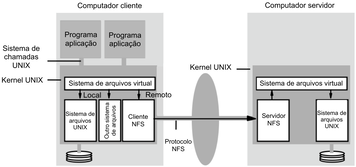
\includegraphics[width=12cm]{arquiteturaNFS.png}
            \caption{Arquitetura do NFS ~\cite{coulouris}}
            \label{fig:arquiteturaNFS}
        \end{figure}
    
    Seu projeto independente do estado do sistema (\textit{stateless}) basicamente inviabiliza a utilização de mecanismos para recuperação de falhas ~\cite{coulouris}.
    
    O uso de memória \textit{cache} no servidor tenta antecipar o que o cliente irá solicitar e já manter esses dados na memória para que, quando o cliente solicitá-los, possam ser entregues sem o gargalo de acesso ao disco. O uso de \textit{cache} na escrita se baseia em manter o arquivo na memória por um tempo sem que o cliente o altere e só então gravar o arquivo no disco. Ainda sim existe a operação \textit{sync} que grava as informações pendentes no disco a cada 30 segundos.
    Quanto a \textit{cache} no cliente é feita através da datas de modificação dos arquivos. Caso haja discrepâncias entre cliente e servidor, o cliente é atualizado ~\cite{coulouris}.
    
    Para questões de segurança o NFS utiliza dois mecanismos externos. Para a transmissão dos dados, autenticação e comunicação do cliente com o servidor é utilizado o protocolo Kerberos v5 junto com RPCSEC\_GSS. Para proteger os dados nos clientes é utilizado a lista de controle de acesso (ACL) que é responsável por definir as permissões para acesso aos arquivos. ~\cite{tanenbaum}.
    
    Quanto a desempenho, o NFS fornece uma solução satisfatória até mesmo para sistemas com grande demanda, ao utilizar diversos servidores. Mas essa solução é limitada pelo fato do sistema não fornecer suporte a replicação de arquivos para leitura e escrita (apenas a replicação para leitura é suportada). Ainda sim, mesmo que bastante difundido e utilizado o NFS carece de mecanismos de migração de dados e réplicas que estão presente em outros SAD mais avançados ~\cite{coulouris}.
    


    \subsection{\textit{Andrew File System} (AFS)}

   
    Da mesma forma que o NFS visto na sessão anterior, o \textit{Andrew File System} (AFS) além de ser compatível com o NFS também fornece acesso de forma transparente aos arquivos, embora utilize uma abordagem um pouco diferente para atingir esse objetivo. Tendo como objetivo principal a escalabilidade do sistema seus mecanismos de cache no cliente são bem agressivos e nas versões mais atuais o sistema passou a trabalhar armazenando o estado dos clientes com o uso de de \textit{callbacks} para diminuir a comunicação entre cliente e servidor e manter baixo o uso dos processadores nos servidores como apresentado por ~\cite{coulouris}.
    
    O AFS tem seu projeto baseado na suposição sobre o tamanho médio e máximo dos arquivos em discos nos sistemas \textit{UNIX} de ambientes acadêmicos e outros. De acordo com ~\cite{coulouris} as observações mais importantes sobre a implementação do AFS são:
    \begin{itemize}
        \item Os arquivos costumam ser pequenos (normalmente com menos de 10KiB).
        \item Operações de leitura são muito mais frequentes que as de escrita (6 vezes mais recorrentes).
        \item O acesso aos arquivos é feito de forma sequencial na maioria das vezes.
        \item A maioria dos arquivos é lida e escrita por apenas um usuário, e mesmo quando compartilhado a maioria das vezes apenas um único usuário é responsável por escrever no arquivo.
        \item Os arquivos tendem a ser referenciados repetidas vezes em momentos próximos.
    \end{itemize}
    
    Com base nessas premissas o AFS opera da seguinte forma:
    \begin{itemize}
        \item Servir arquivos inteiros.
        \item Cache de arquivos inteiros nos clientes.
        \item Uso de cache persistente nos clientes (armazenados em disco).
        \item Uso de um kernel modificado nos clientes para interceptar as chamadas de acesso aos arquivos.
    \end{itemize}
    
    Com base nos estudos feitos e nas características citadas acima é fácil perceber que existe um grupo de arquivos que é totalmente fora desse escopo: arquivos de bancos de dados. Dessa forma o projeto do AFS declaram explicitamente que o objetivo do sistema não é atender a essa categoria de arquivos.
    
    A arquitetura do AFS utiliza servidores e clientes. O \textit{software} utilizado nos servidores é chamado de Vice, enquanto o que executa nas estações clientes é o Venus, como pode ser visto na Figura \ref{fig:arquiteturaAFS} .
    
    \begin{figure}[h]
        \centering
        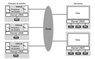
\includegraphics[width=12cm]{arquiteturaAFS.png}
        \caption{Arquitetura do AFS ~\cite{coulouris}}
        \label{fig:arquiteturaAFS}
    \end{figure}
    
    O gerenciamento de cache no cliente é tratado pelo processo Venus, que ao receber uma operação open verifica se o arquivo solicitado já existe na cache e se existe alguma versão mais nova desse arquivo nos servidores. Caso o arquivo da cache esteja defasado a nova versão é solicitada aos servidores e é fornecida ao programa que fez solicitou o arquivo. Quando o arquivo é fechado através da operação \textit{close} o processo Venus (cliente) verifica se o arquivo foi alterado e caso afirmativo envia a nova versão do arquivo ao servidor. É importante ainda ressaltar que o AFS não dispõe de nenhum mecanismo para tratar atualização concorrente de um mesmo arquivo, de forma que se vários clientes enviarem versões diferentes do mesmo arquivo ao servidor, todas exceto a última a ser processada pelo servidor (Vice) serão perdidas sem nenhum aviso ou erro, restando apenas a última requisição processada pelo servidor, que será a versão do arquivo que será salva e estará disponivel ~\cite{coulouris}.
    
    Quanto aos metadados vale citar que os banco de dados ficam replicados integralmente em todos os servidores (Vice) ~\cite{coulouris}, de forma que cada servidor sabe exatamente onde se encontram os arquivos.
    
    Semelhante ao NFS, o AFS só suporta réplica de arquivos para leitura, direcionando todas as escritas nesse arquivo para apenas um servidor, que então faz o sincronismo posteriormente e tem que ser feita de forma explicita ~\cite{coulouris}.
    
    As características citadas acima fornecem ao AFS um bom desempenho para cargas relativamente grandes sem sobrecarregar demasiadamente os servidores, o que fornece grande taxa de escalabilidade, sendo em alguns casos até 60\% mais eficiente no uso de CPU que o NFS com a mesma carga de trabalho ~\cite{coulouris}.
  

    
    %\subsection{\textit{Tahoe-LAFS- Least Authority File System}}
    %Escrever.   
    %\subsection{CODA \textit{Distributed File System}}
    %Escrever.
    %\subsection{\textit{Hadoop File System}}
    %Escrever.
                                            
    \subsection{\textit{Flexible and Adaptable distributed file system} (FlexA)} \label{flexa}
	 
	 O \textit{Flexible and Adaptable distributed file system} (FlexA) ~\cite{silas}, desenvolvido pelo Grupo de Sistemas Paralelos e Distribuídos (GSPD) que é o objeto de estudo desse trabalho, tem foco na utilização de recursos computacionais das estações clientes para diminuir a carga de processamento dos servidores, além de fornecer um sistema de segurança descentralizado e o uso de mecanismo de tolerância a falhas, aproveitando características de diversos SADs, focando em fornecer um SAD com grande escalabilidade ~\cite{silas}.
	
	 O FlexA mudou muito desde sua versão inicial, desenvolvida em 2012 ~\cite{mario}. A versão que será tratada nesse texto é a última versão que ainda está em desenvolvimento, baseada na versão original. Essa versão é o resultado da cooperação de diversos integrantes do GSPD ~\cite{mario}, durante a evolução do sistema nesses dois anos desde sua versão inicial. A arquitetura do sistema original pode ser vista na Figura \ref{fig:arquiteturaFlexaSilas} .
	 
	 \begin{figure}[!ht]
	 \centering
	 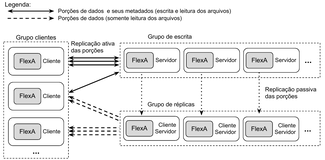
\includegraphics[width=14cm]{arquiteturaFlexAOriginal.png}
	 \caption{Arquitetura original do FlexA ~\cite{silas}.}
	 \label{fig:arquiteturaFlexaSilas}
	 \end{figure}
	 
	 A arquitetura atual do projeto, se baseia muito no que foi proposto por ~\cite{silas} é apresentada na Figura \ref{fig:arquiteturaFlexaMario}.
	 
	 \begin{figure}[!ht]
	 \centering
	 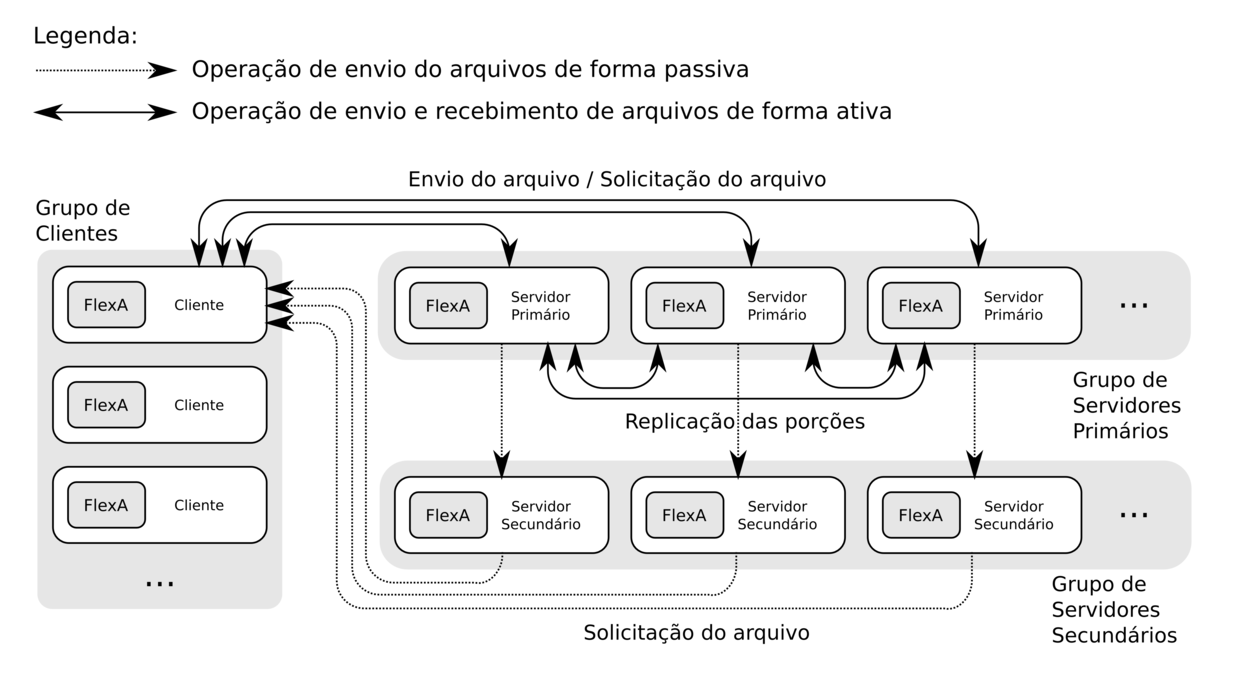
\includegraphics[width=14cm]{arquiteturaFlexA.png}
	 \caption{Arquitetura atual do FlexA ~\cite{mario}.}
	 \label{fig:arquiteturaFlexaMario}
	 \end{figure}
	 
	 Além disso a distribuição dos arquivos também foi alterada, para que o sistema apresente um desempenho melhor do lado cliente, a replicação das porções dos arquivos na fração de 2/3 em cada servidor primário fica agora na responsabilidade dos servidores primários. o diagrama apresentado na figura \ref{fig:arquivosSilas} mostra como era a movimentação dos dados no FlexA original, e a figura \ref{fig:arquivosMario} mostra a nova versão ~\cite{mario}.
	 
	 \begin{figure}[!ht]
	 \centering
	 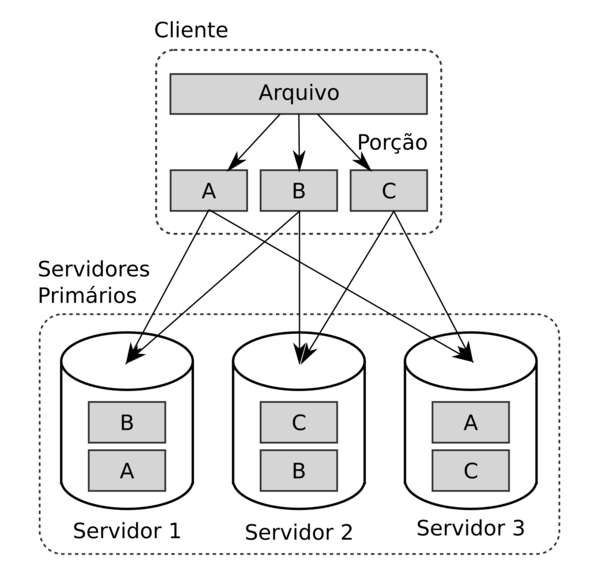
\includegraphics[width=10cm]{arquivosFlexaSilas.png}
	 \caption{Fluxo de dados no FlexA original ~\cite{silas}.}
	 \label{fig:arquivosSilas}
	 \end{figure}
	 
	 \begin{figure}[!ht]
	 \centering
	 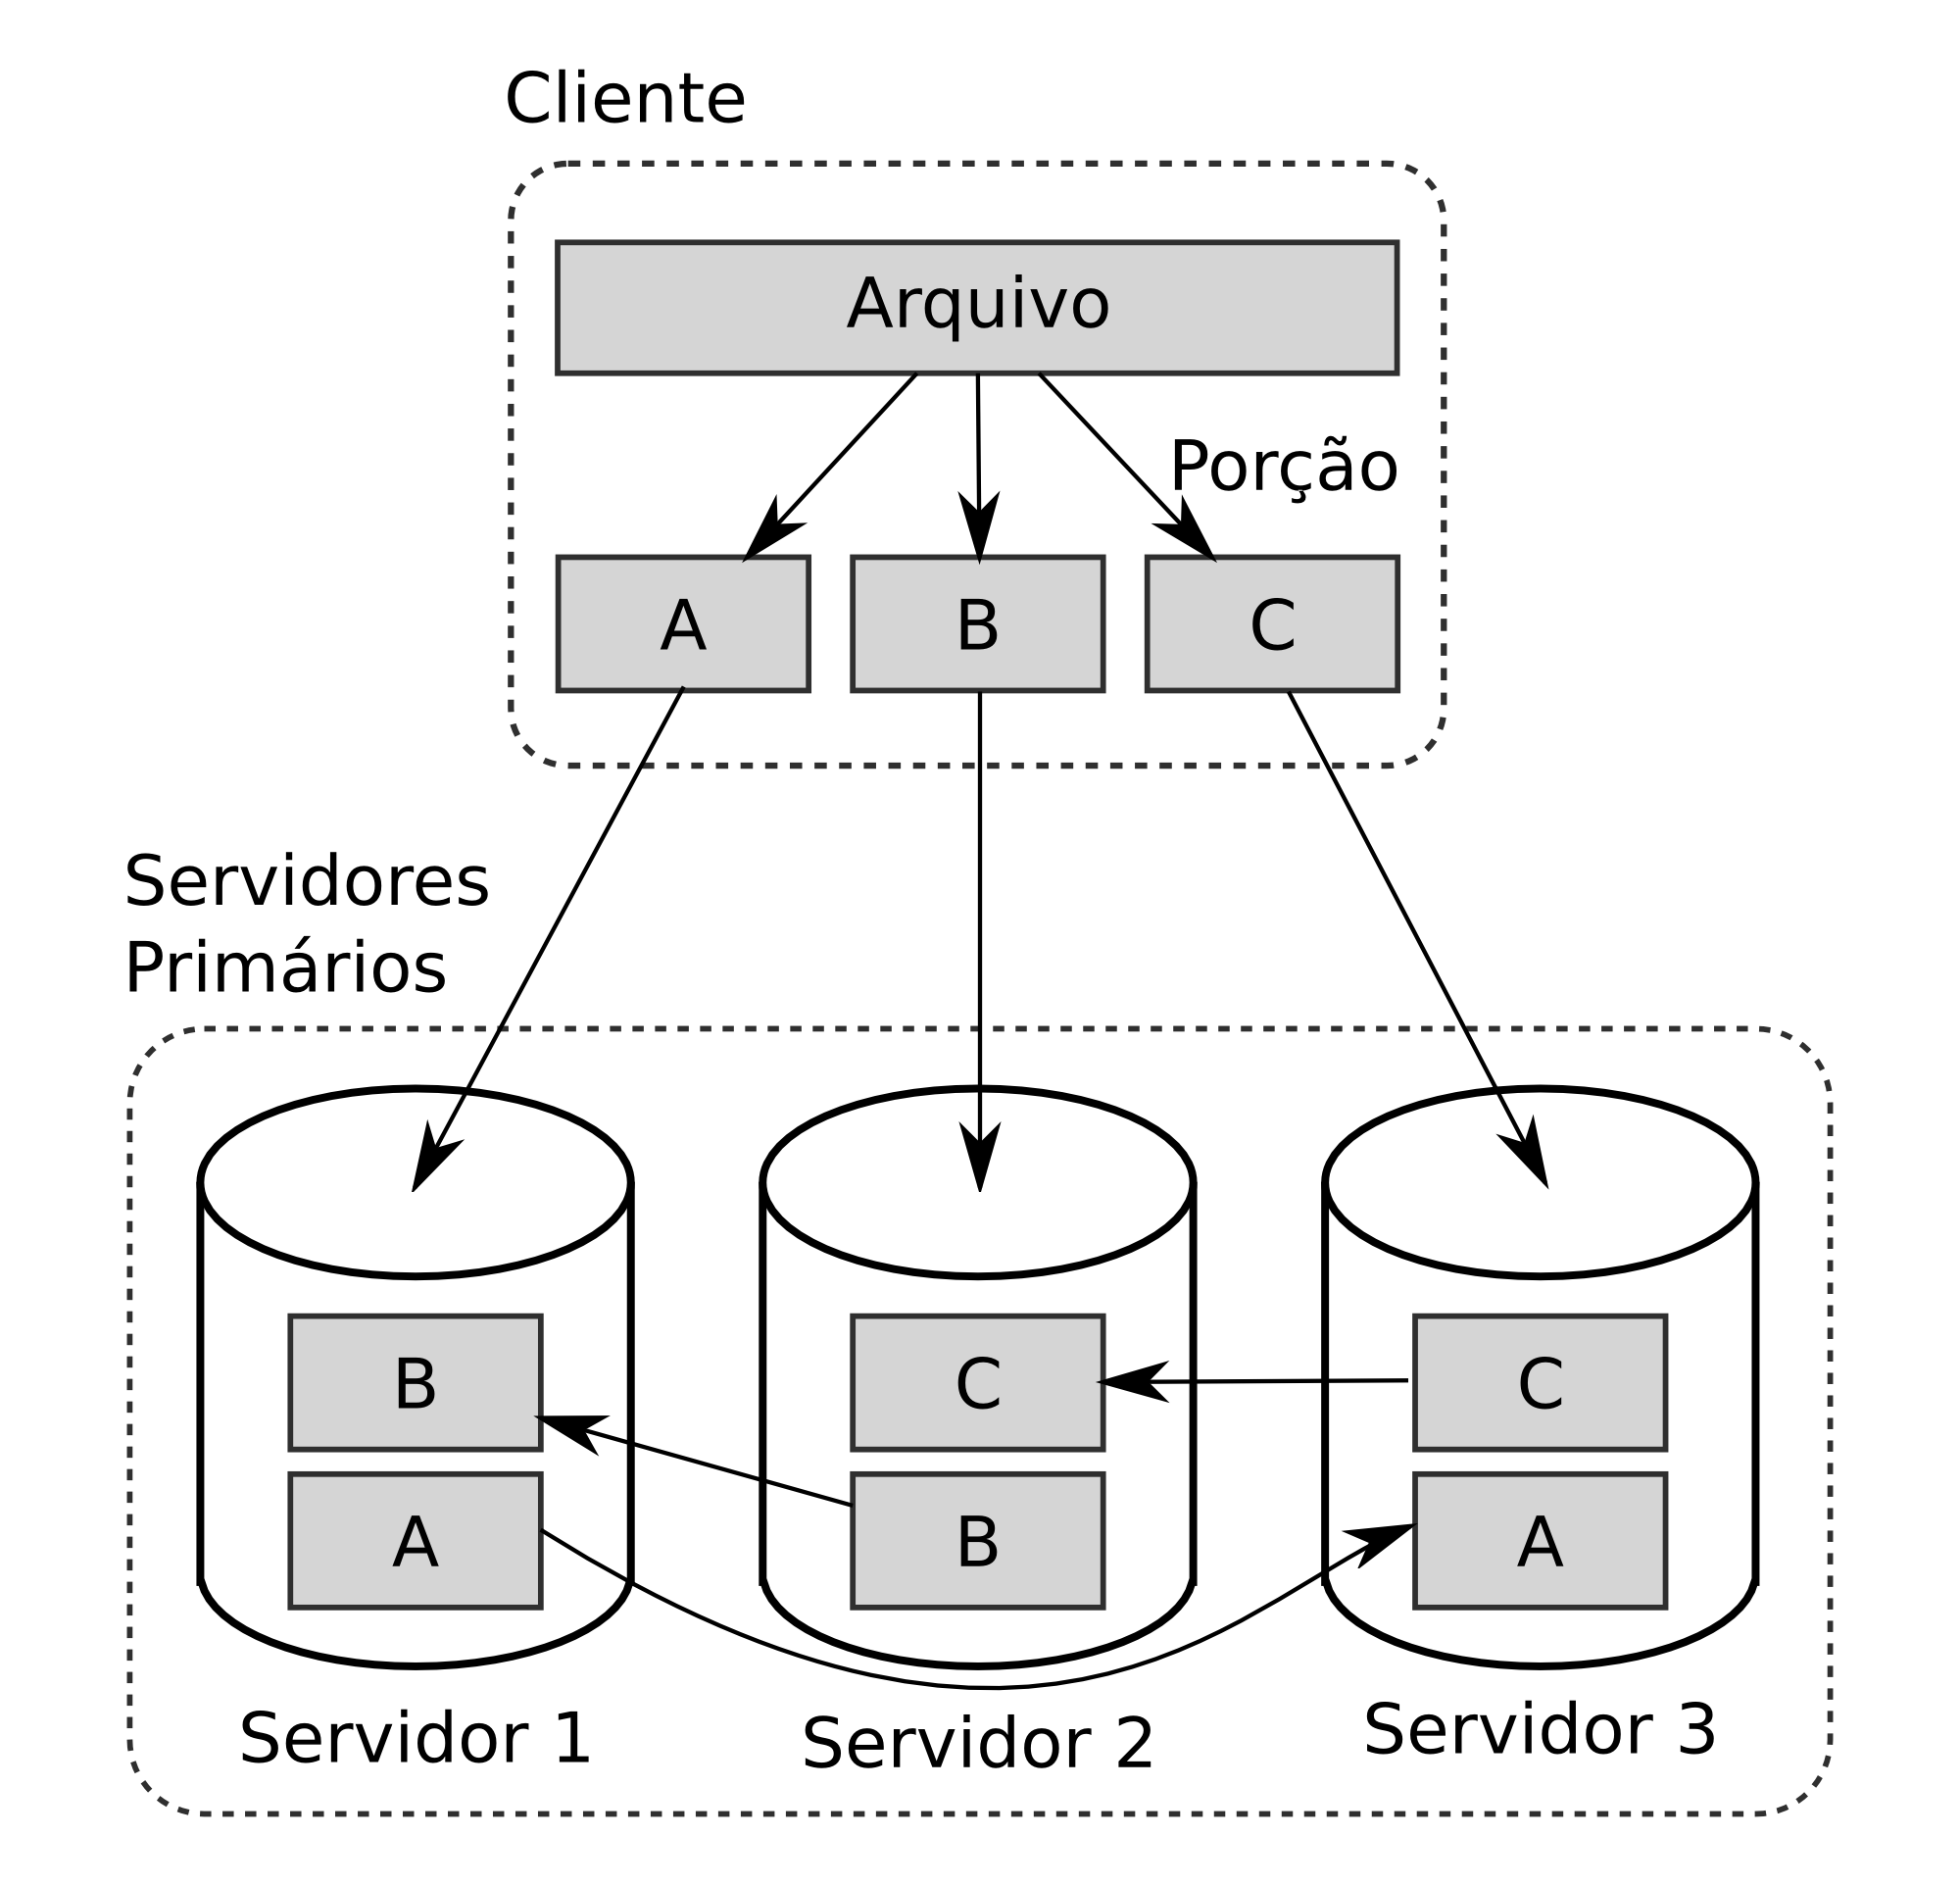
\includegraphics[width=10cm]{arquivosFlexaMario.png}
	 \caption{Fluxo de dados no FlexA atual, elaborado a partir de ~\cite{mario}.}
	 \label{fig:arquivosMario}
	 \end{figure}
	 
	 
	 Para atingir os objetivos descritos acima o FlexA possui diversos mecanismos que serão elencados nas sessões a seguir.
	 
	 \subsection{Segurança}
	    A segurança do sistema é baseada no controle de acesso aos arquivos e também no controle de escrita sobre o mesmo ~\cite{silas}.
	 
    	 \begin{itemize}
    	 
    	    \item Controle de Acesso: é implementado utilizando um trio de chaves para cada arquivo. As chaves que compõe esse trio são:
        	    \begin{itemize}
        	        \item \textit{Verify Key} (VK): fornece acesso ao arquivo, servindo como um identificado único do arquivo no sistema.
        	        \item \textit{Read Key} (RK): é a chave utilizada para cifrar o arquivo. Sem essa chave, mesmo que seja conhecida a VK não é possivel ler o conteúdo do arquivo.
        	        
        	        \item \textit{Write Key} (WK): fornece acesso de escrita no arquivo dentro dos servidores.
        	    \end{itemize}
        	    
            Das três chaves citadas acima a única que não é enviada aos servidores é a chave usada na criptografia do arquivo, a \textit{Read Key}. Dessa forma mesmo que o servidor seja comprometido não é possível obter o conteúdo original dos arquivos que ele armazena ~\cite{mario}.
        	    
        	    
        	    Essas chaves são criadas com base em uma chave privada RSA ~\cite{shamirRSA} especificada pelo usuário, junto com um valor único para cada arquivo chamado de \textit{salt} que é fornecido pelo servidor. Uma vez com a RSA e o \textit{\textit{salt}} o processo feito para obtenção do trio de chaves é o apresentado na Figura \ref{fig:chavesFlexa}.
        	    
        	    \begin{figure}[!ht]
        	    \centering
        	    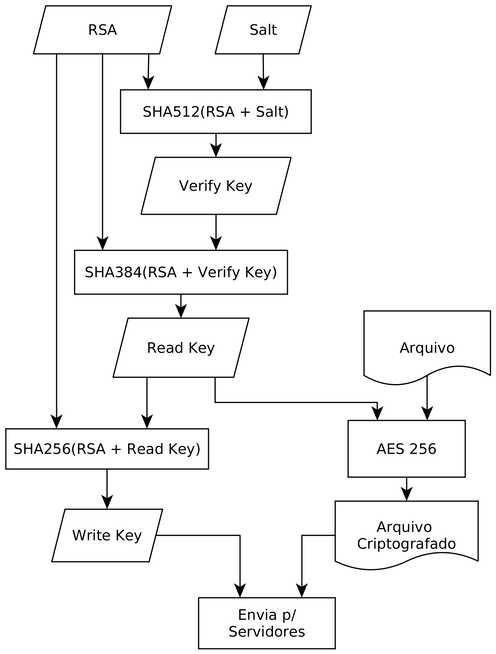
\includegraphics[width=10cm]{chaves.png}
        	    \caption{Diagrama sobre a criação das chaves de acesso e criptografia do FlexA ~\cite{mario}.}
        	    \label{fig:chavesFlexa}
        	    \end{figure}
        	    
        	    Como mostrado na Figura \ref{fig:chavesFlexa} a chave de identificação do arquivo (VK) é gerada utilizando a o \textit{hash} SHA512 da RSA do usuário concatenada com o do \textit{salt} retornado pelo servidor.
        	    Após isso a chave de criptografia (RK) é gerada utilizando a o hash SHA386 da RSA do usuário concatenada com o do identificador do arquivo (\textit{Verify Key});
        	    Por fim é gerado a chave de escrita (WK), utilizando a RSA do usuário concatenada com a chave de leitura.
        	    
        	    Todo o processo criptográfico e de geração de chaves é feito de forma transparente, sem que o usuário tenha que fazer isso de forma manual, notando apenas o tempo que é necessário para fazer a criptografia / descriptografia do arquivo.
    	    
        \item Integridade: O mecanismo de integridade do arquivo é implementado utilizando a chave WK mostrada anteriormente. A permissão de escrita (chave WK) é solicitada sempre que um cliente deseja fazer a operação de escrita (atualização) de um arquivo nos servidores. Dessa forma o cliente deve fornecer a WK correspondente ao arquivo que deseja atualizar, então o servidor comprara a WK fornecida com a armazenada e caso sejam idênticas o servidor faz a substituição do arquivo antigo pelo novo.
        
        Mecanismos para evitar ataques de repetição e outros semelhantes ainda precisam ser implementadas no FlexA, pois a transmissão das chaves de acesso e escrita podem ser facilmente capturadas e reutilizadas com a implementação atual.
        
    \end{itemize}
    
    \subsection{Tolerância a falhas e Adaptabilidade}
        
        Os mecanismos utilizados pelo FlexA para executar esse objetivo são o uso de réplicas das porções dos arquivos, que são enviados para diversos servidores e lá são replicados com o grupo de servidores secundários. Também é utilizada a possibilidade de um servidor secundário assumir além da sua função a de um servidor primário caso seja necessário por falha de algum primário ou sobrecarga do grupo de servidores primários ~\cite{mario}.
        
        Sempre que um servidor primário ou secundário falha, é executado um processo que faz o sincronismo do servidor com os outros servidores ativos para que esse assuma o estado atual do sistema e volte o mais breve possível a colaborar com o atendimento dos clientes ~\cite{silas}.
        
    
    \subsection{Escalabilidade}
    
        Os principais fatores que auxiliam na escalabilidade do sistema são:
        
        \begin{itemize}
            \item Criptografia e descriptografia dos arquivos nos clientes: Evitam o consumo de UCP nos servidores, deixando-os mais disponíveis para atender a novas requisições.
            \item Divisão dos arquivos em diversas porções nos clientes: Diminuem o uso de armazenamento e uso dos discos dos servidores.
            \item União das diversas porções que compõe um arquivo nos clientes: Também influenciam no uso de disco dos servidores, liberando os discos para atenderem outras requisições mais rapidamente.
            \item Leitura e escrita das porções dos arquivos de diferentes servidores, evitam sobrecarregar o uso de banda de apenas um servidor e aumentam o uso da banda no cliente.
            \item Utilização agressiva de cache nos clientes: Essa técnica evita acessos recorrentes aos servidores, principalmente para arquivos que são pouco atualizado ou são utilizados por apenas um usuário.
            \item Uso de sistemas de replicação para servidores secundários: Auxiliam nas operações de leitura dos arquivos pelos clientes.
        \end{itemize}
        
        
    \subsection{Flexibilidade}
    
        Como boa parte da carga de processamento e uso do disco no FlexA é transferida aos clientes, o sistema pode operar com \textit{hardware} de baixo custo sem grandes problemas. Isso ainda fornece ao FlexA a possibilidade de que caso seja necessário clientes com mais recursos disponíveis podem passar a fazer parte do grupo de servidores auxiliando no atendimento a requisições de outros clientes. Essa característica faz com que o sistema aproveite muito recurso que estaria ocioso em sua rede, principalmente em momentos de uso intensivo dos servidores ~\cite{silas}.
        
        Além disso o sistema é projetado para que seja possível fazer a troca dos mecanismos de segurança, regras de gerenciamento da cache nos clientes,  métricas de divisão das porções e diversos outros elementos do sistema de forma simples, principalmente devido a escolha do Python como linguagem de programação, facilita o acesso ao código fonte do FlexA ~\cite{silas}.
        
    \subsection{Abertura}
    
    A abertura do FlexA é dada basicamente pelo fato de o sistema ter o código fonte aberto e disponível ~\cite{silas}, sendo necessário aprimorar a documentação existente. 


\section{Chamada de Procedimentos Remotos (RPC)}

    Para realizar comunicação entre cliente e servidores é possível utilizar diversas técnicas diferentes. Nesse trabalho a Chamada de Procedimento Remoto ou \textit{Remote Procedure Call} (RPC) é uma ferramenta muito utilizada pois é a partir dela que a maior parte das comunicações entre cliente e servidor acontecem. A escolha desse paradigma foi feita pela simplicidade do projeto e desenvolvimento. 
    
    O RPC utiliza um paradigma de comunicação de alto nível, ocultando do desenvolvedor quase todo o processo de estabelecimento de conexão, transmissão dos dados, conversão dos dados e bloqueio do cliente ~\cite{rpc} ao realizar requisições.
    
    A descrição básica da comunicação via RPC é feita em ~\cite{rpc}. Para a utilização do RPC na implementação de um serviço é necessário um processo chamado de servidor RPC (Servidor) que possui as funções disponíveis que serão solicitadas por um cliente através de uma requisição RPC. Assim cabe ao Servidor registrar todas as funções que o cliente pode requisitar. Após registrar as operações o Servidor inicia a escuta por requisições.
    
    Em outro \textit{host}, um processo chamado Cliente faz uma Requisição RPC ao Servidor. O Servidor executa a função solicitada, com os parâmetros enviados e retorna o resultado ao cliente.
    
    De acordo com ~\cite{rpc} o uso de RPC reduz em média 50\% da complexidade no desenvolvimento da comunicação entre cliente e servidor.
    
    \subsection{XML-RPC}
    
    No mercado existem diversas soluções para o uso de RPC. O XML-RPC é uma implementação de RPC que utiliza TPC/IP junto com HTTP e XML para a troca de mensagens entre servidor e cliente ~\cite{xmlrpc}. O uso de um padrão como o XML-RPC é também justificado pela representação dos dados que é mantida através de diversas arquiteturas ~\cite{xmlrpcMessage}
    
    A versão atual do FlexA utiliza o XML-RPC para todas as comunicações entre cliente/servidor exceto para a transmissão de arquivos ~\cite{mario}. A transmissão dos arquivos é feita via \textit{socket} para evitar o processo de \textit{marshalling} dos arquivos que tende a ser demasiadamente custoso em questões de uso de UCP e demorado, dessa forma reduzindo o tempo de entrega dos arquivos ao cliente.
    
    Um diagrama bem simples sobre o funcionamento desse paradigma descrito acima é exibido na Figura \ref{fig:xmlrpc}.
    
    \begin{figure}[!ht]
    \centering
    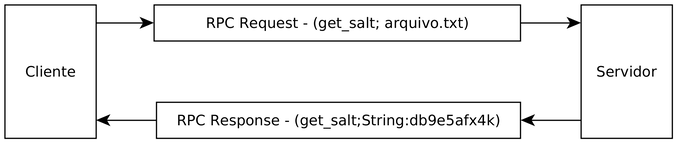
\includegraphics[width=10cm]{xmlrpc.png}
    \caption{Diagrama que exibe a comunicação via XML-RPC. ~\cite{xmlrpc} (Adaptado)}
    \label{fig:xmlrpc}
    \end{figure}
    
    Como pode ser visto na \ref{fig:xmlrpc}, o cliente faz a requisição de uma função remota, passando os parâmetros. Toda a comunicação é feita com o uso de XML. O servidor recebe a requisição, processa e retorna o resultado também em XML. Um outro exemplo mostra como é feita a comunicação de uma requisição com XML-RPC como pode ser visto na Figura ~\ref{fig:xmlrpcMessage} . O processo de resposta da requisição segue o mesmo principio.
    
    \begin{figure}[!ht]
    \centering
    \fbox{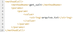
\includegraphics[width=10cm]{xmlrpcMessage.png}}
    \caption{Exemplo de mensagem XML utilizada na chamada de procedimentos remotos com XML-RPC.}
    \label{fig:xmlrpcMessage}
    \end{figure}


\section{Dispositivos Móveis}

    Quanto a classificação de dispositivos móveis, é muito difícil fornecer uma definição formal que seja adequada. Assim essa definição pode ser feita em duas partes, como feita em ~\cite{mobileDevices}.
    
    \subsection{Dispositivos Móveis}
    De acordo com ~\cite{mobileDevices}, dispositivos móveis são dispositivos portáveis como    \textit{laptops}, \textit{Personal Digital Assistants} (PDA), \textit{tablets}, \textit{smart phones}, \textit{handhelds}, \textit{MP3 Players}, consoles de jogos portáteis entre outros. Variando de dispositivos com pouquíssima autonomia, baixa ou nula conectividade e pouca capacidade computacional até dispositivos de ultima geração com autonomia relativamente alta (algumas dezenas de horas de uso constante), potência computacional muitas vezes superior a computadores de mesa e \textit{notebooks} e grande conectividade utilizando diversas tecnologias diferentes. 
    
    
    \subsection{Computação Móvel}
    Dentro do escopo desse trabalho mais importante que a definição de dispositivos móveis é a definição  computação móvel, que é apresentada por ~\cite{mobileDevices} como sendo um conjunto de dispositivos móveis que fornecem ao usuário um sistema computacional que pode operar em dois modos: conectado e desconectado. Quando desconectado de redes de dados esses dispositivos devem funcionar de forma dessincronizada com sua fonte de dados, e quando conectados novamente a redes que fornecem acesso a transmissão de dados devem fazer o sincronismo dos dados através de operações de \textit{upload/download}.
    
    
\section{Android}

Na maioria das vezes é necessário um sistema operacional (SO) que gerencie um dispositivo móvel, esse sistema operacional pode ser o Android ~\cite{android} ou outro sistema operacional comum ou preferencialmente próprio para dispositivos desse tipo. Existem atualmente no mercado dezenas de SOs diferentes para dispositivos móveis, mas os que mais se destacam frente aos usuários e grandes fabricantes são Android (\textit{Open Handheld Alliance}) e iOS (Apple) ~\cite{mobileDevicesMarketShare}.

Mais do que um simples sistema operacional, o Android é composto por diversas camadas de software (~\textit{Android Software Stack}) que fornecem ao sistema suporte a uma grande variedade de dispositivos e flexibilidade no seu uso ~\cite{android}. Essas camadas são exibidas na Figura \ref{fig:androidStack}.

\begin{figure}[h]
\centering
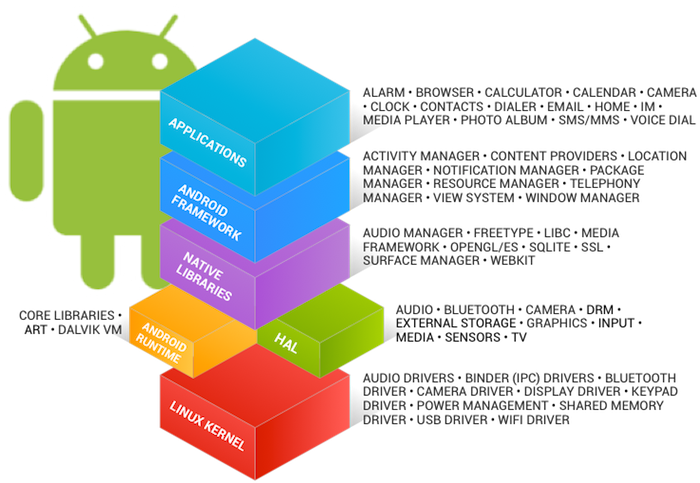
\includegraphics[width=14cm]{androidStack.png}
\caption{Camadas de software que compõe o sistema Android ~\cite{android}.}
\label{fig:androidStack}
\end{figure}

